\documentclass[journal,final,a4paper,twoside]{PS}

%%% Dieser Block ist dem Betreuer des Projektseminars vorbehalten
\usepackage{PS}             % Alle Definitionen �ber den Seitenstil (auf keinen Fall editieren!!)
\usepackage[T1]{fontenc}
\usepackage[utf8]{inputenc}
\usepackage{tikz}
\usepackage[]{algorithm2e}
\usepackage{svg}
\usepackage{amsmath}
\def\lehrveranstaltung{PROJEKTSEMINAR ROBOTIK UND COMPUTATIONAL INTELLIGENCE}
\def\ausgabe{Vol.17,~SS~2017}
\setcounter{page}{1}        % Hier die Seitennummer der Startseite f�r Gesamtdokument festlegen
%\bibliographystyle{unsrt}

%%% Ab hier k�nnen Eintr�ge von den Teilnehmern des Projektseminars gemacht werden
%%% Wenn neben den LaTeX-Paketen aus der Datei PS.sty noch weitere gebraucht werden,
%%% so ist dies dringend mit dem Betreuer abzukl�ren!

\begin{document}
\newcommand{\euertitel}{Dynamic Distortion Calibration}   % Titel hier eintragen!
\newcommand{\betreuer}{M. Sc. Raul Acu\~na }  % Betreuerdaten hier eintragen (mit einem Leerzeichen am Ende)!


\headsep 40pt
\title{\euertitel}
% Autorennamen in der Form "Vorname Nachname" angeben, alphabetisch nach Nachname sortieren,
% nach dem letzen Autor kein Komma setzen, sondern mit \thanks abschlie�en
\author{Ahmed Ashraf,
        Nils Hamacher,
        Linghan Qian,
	Vivica Wirth
\thanks{This paper was supported by \betreuer.}}

\maketitle


\begin{Zusammenfassung}
Kameras als Sensoren werden in immer mehr Applikationem im allt\"aglichen Leben wie zum Beispiel in Smartphones, oder um unser Haus mit Hilfe von Smart-Home-Systemen zu \"uberwachen, verwendet. In Fabriken hingegen werden noch viel mehr Kameras zur \"Uberwachung von verschiedensten Prozessen wegen ihrer universellen Anwendung, niedrigen Kosten und dem Potenzial der erhaltenen Daten verwendet. Au\ss{}erdem w\"achst ihre Rolle im Automobilbereich. Jedoch ist jede Kameralinse aufgrund von nicht exakt gleichm\"a\ss{}igen Fertigungstechniken mehr oder weniger gekr\"ummt. Die meisten Kameras zeigen eine radiale Verzerrung, da die Linsen in der Regel eine konvexe Kr\"ummung aufweisen. Diese ist nicht immer gleichm\"a\ss{}ig konvex oder hat Einschl\"usse, die die Verzerrung zu einem sehr nichtlinearen Verhalten ver\"andert. Das macht die Kalibrierung des Kameraobjektivs zu einem wesentlichen Aspekt der Computer Vision, da eine hohe Genauigkeit ihrer Bilder erforderlich ist. Die meisten Kamerakalibrierungen erfordern menschliche Interaktionen wie die Kalibrierung mit einem Schachbrettmuster. In dieser Ausarbeitung wird eine L\"osung f\"ur die Kamera-Kalibrierung vorgestellt, die auf einem planaren Display wie g\"angigen Computermonitoren arbeitet und nicht auf menschliche Interaktion st\"utzt. Dabei wird eine Karte zwischen den Bildschirmpixeln und den projezierten Karmerabildpixeln bestimmt. Wir pr\"asentieren verschiedene Wege, die wir mit ihren Vor- und Nachteilen in Genauigkeit und Laufzeit ausprobiert haben.
\end{Zusammenfassung}
\vspace{6pt}

\begin{abstract}
Cameras as a sensor application are widely used in our daily life like in smartphones or to surveille our home via smart home installation. But even more cameras monitor many processes in factories because of their universal application, low cost and the potential of the obtained data. Also it influence in the automotive branche is rising. However, every camera lens is more or less distorted due to imperfect manufacturing techniques. Most cameras show radial distortion due to the fact that most lenses have convex curvature. These aren't always perfectly convex or got inclusions which do alter the distortion to a very non-linear behavior. That makes calibration of the camera lens an essential aspect of computer vision, since a high accuracy of their images is required. Most camera calibrations require human interactions like the calibration with a checkerboard. In this paper a solution to camera calibration is shown that works on a 2D planar display like common used computer monitors and doesn't rely on human interaction. Therefore a mapping between the screen pixel coordinate system and the image pixel coordinate system is determined. We present different ways we tried with their pros and cons in accuracy and runtime.
\end{abstract}

\section{Introduction}

\PARstart{C}{ameras} are used in more and more situations. Application areas are monitoring technologies, toys, smartphones and increasingly in vehicles for example. However all camera lenses are somewhat different from each other. The curvature of a lens is never perfect, and inclusions may occur which also alter the curvature of the incident light. This leads to distortion that has to be calibrated. State of the art approaches like the checkerboard calibration only base their models on a few interest points. This method for calibration is to position a checkerboard in different poses in front of the camera and detect the intersections of the black and white squares. The more pictures are done the higher is accuracy of the result what increases the human interaction and the time invested. We present this and other methods in Chapter \ref{sec:related}. 
Our aim was to develop a program, which automatically creates a dense model of the lens distortion. This dense model is based on information of the correspondencies of pixels on a screen and the pixels in a captured image. Once the mapping between the screen and the image corresponding pixels is done, we can undistort the image simply by moving the pixels of the actual image we take. In order to reach the desired accuracy we need to set some pre-conditions for the environment in which this takes place. These conditions are darkness, in order to avoid reflections of the camera on the screen, and the camera being perpendicular to the screen. We will present the fundamental principles of several different ideas, which all result in a mapping. To compare them we give a short insight to their runtimes. This article is structured as follows: First follows the related work in \ref{sec:related} then in Chapter \ref{sec:maths} the theoretical  foundations are outlined. Chapter \ref{sec:mapping} includes the idea and realization of the project. In Chapter \ref{sec:results} is the conclusion.


\subsection{Related Work}
\label{sec:related}
Several approaches has been proposed in order to calibrate a camera, they can roughly be classified into two categories \cite{Zhang}: photogrammetric calibration and self-calibration.
Photogrammetric calibration is based on a spatial object with its $3D$ shape known which is placed in the view of camera. The commonly used object is planar object point array, so called checkerboard pattern \cite{Zhang}, or a $3D$ cube with determined pattern on it. This method is restricted because errors will occur while printing and manually measuring the pattern or also if the pattern isn't always available.\\
In self-calibration \cite{Faugeras} a reference object is not required, instead it requires the correspondence between points of the scene and the projection. C.B.~Duane proposed in \cite{Duane} a nonmetric method, based on the fact that the projection of a straight line from the world space should also be a straight line on the image. R.~Swaminathan and S.K.~Nayar extended in \cite{Swaminathan} this method by reducing noise and using polycamera. However, this method still relies on calculating parameters, which is not accurate because the model is simplified. 
In \cite{Sagawa} a way is proposed using structured light to determine the correspondence and creates directly a dense map so that the error generated by parameter fitting is reduced. 
The system proposed is based on \cite{Sagawa} since they are both based on detecting the correspondence of lines and get the map non-parametrically. %\cite{Faugeras:1992}

\section{Mathematical Backround}
\label{sec:maths}







\section{Image formation in digital camera}
\label{sec:imageFormation}
The first thing of human perception of the world is observing through eyes or cameras for robots. Through that a lot of information will be gathered, like size, shape and distance of objects in the world, in conjunction with many object characteristics like color and texture, that leads to recognition of things.
All creatures, that can see, have a lens that forms an inverted image on the retina where the light sensitive cells rod and cone cells, are arranged. A digital Camera is like human eye in principle, a lens, which can be made from glass or plastic, forms an Image on the surface of semiconductor chip with an array of light-sensitive devices to convert light to digital image.

The formation of Image in an eye or digital camera, is based on the process of a projection of 3D objects onto 2D surface. The transformation from 3D to 2D is known as perspective projection. Through that Projection, the depth information is lost and we cannot tell anymore from image whether it is of a large object in the distance or a smaller close object.

In this section, we will discuss how camera works, images are captured and formed.

\subsection{Perspective projection}
The Pinhole camera idea is based on the principle of perspective projection and it works when a small hole in the wall of a closed box will cast a dim inverted image of the outside world on the opposite side of the box.
\begin{figure}[h]
\begin{center}
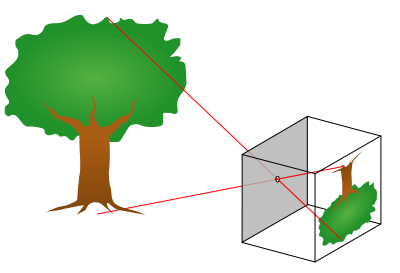
\includegraphics[scale=0.4]{./pics/pinhole.png}
\caption{Image formation in pinhole camera}
\label{fig:pinhole}
\end{center}
\end{figure}
Convex lenses can do the same work as pinhole and the in the following image we can see the fundamental geometry of image formation for a thin convex lens.
\begin{figure}[h]
\begin{center}
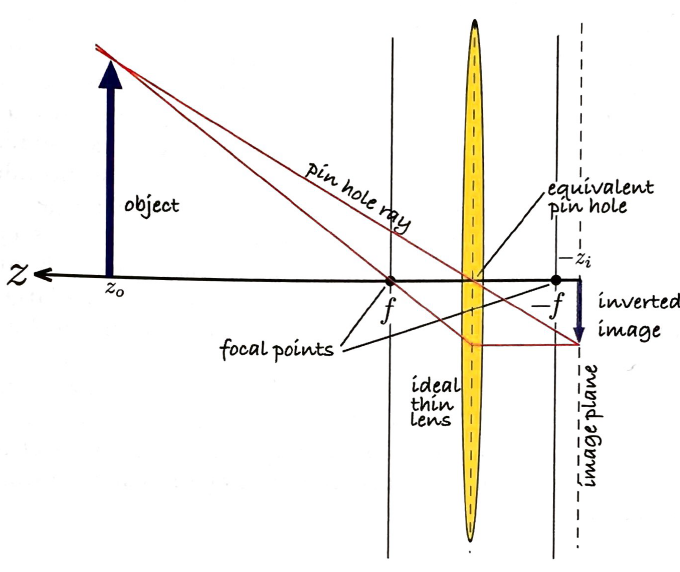
\includegraphics[scale=0.6]{./pics/imageFormationGeometry.png}
\caption{Image formation for a convex lens \cite{Corke}}
\label{fig:imageGeometry}
\end{center}
\end{figure}
The thin lens equation that describes the z-coordinate of the observed object and its image with respect to the CenterPoint of the image \cite{Corke}.
\begin{equation}
\frac{1}{Z_0}+\frac{1}{Z_i}+\frac{1}{f}
\end{equation}



$Z_0$ : the distance to the observed object.

$Z_i$ : the distance to the observed object.

$f$ : is the focal length of the lens.
\\
\\
Its common in Computer vision engineering o use the center perspective imaging model  as shown in the following figure.
\\
%%problem displaying figure here
\begin{figure}[h]
\begin{center}
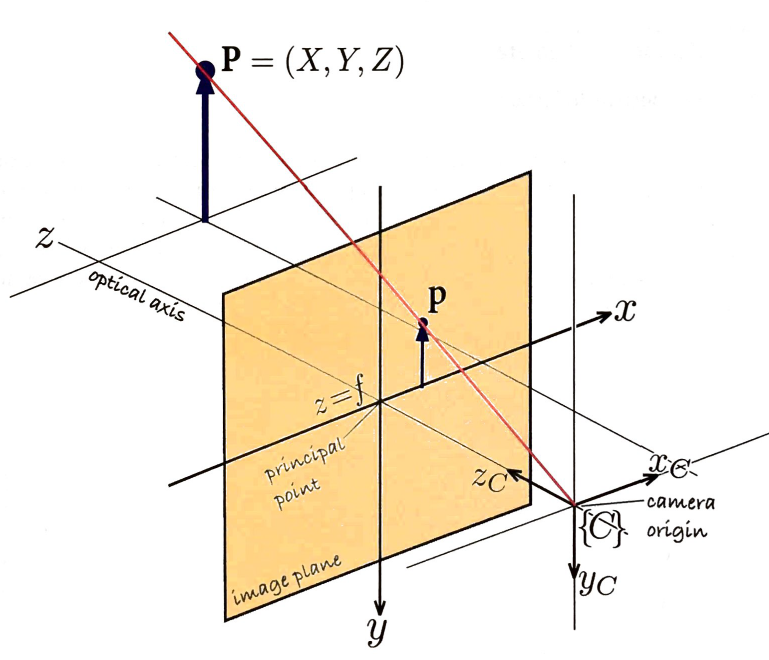
\includegraphics[scale=0.6]{./pics/CenterProjectionModel.png}
\caption{The central-projection model \cite{Corke}.}
\label{fig:projectionModel}
\end{center}
\end{figure}
\begin{subequations}
\begin{align}
\{C\}&\text{ : Origin of camera frame.}\label{eq:C_origin}\\
P_w=(X,Y,Z)^T&\text{ : Point in world coordinates.}\label{eq:P_w}\\
P_i=(x,y)^T&\text{ : Point on the image plane}\label{eq:P_i}
\end{align}
\end{subequations}
The rays of all corresponding Points \ref{eq:P_w} and \ref{eq:P_i} converge all at $\{C\}$ and a noninverted image is projected onto the image plane located art $z=f$. The z-axis intersects the image plane at the principal point which is the origin of the 2D image coordinate frame.
\begin{equation}
x=f\frac{X}{Z}, y=f\frac{Y}{Z}
\end{equation}

Through transformation from the world to image plane, the straight lines in the world are not projected as straight lines on the image plane, parallel lines converge and circles become ellipse, and the size of a shape is not preserved and it depends on the distance.

\subsubsection{Modeling a perspective camera}
By using the homogenous form $\tilde{\textbf{P}}=(\tilde{x} ,\tilde{y} ,\tilde{z} )$ to describe the image-plane point coordinates, where \begin{subequations}\begin{align}
&\tilde{x}=f\cdot X\label{eq:homo_x}\\
&\tilde{y}=f\cdot Y\label{eq:homo_y}\\
&\tilde{z}=Z\label{eq:homo_z}
\end{align}
\end{subequations}


are the homogeneous image-plane coordinate. As well we can formulate it in matrix form\cite{Corke}.
\begin{equation}
\tilde{\textbf{P}} = \begin{pmatrix}
f&0&0\\
0&f&0\\
0&0&1\\
\end{pmatrix}
\begin{pmatrix}
X\\
Y\\
Z\\
\end{pmatrix}
\end{equation}
and
\begin{equation}
x=\frac{\tilde{x}}{\tilde{z}}, y \frac{\tilde{y}}{\tilde{z}}
\end{equation}
are the nonhomogeneous image-plane coordinates.
\\
When $f=1$ the coordinates are referred to as the canonial, retinal or horizontalized image-plane coordinate and we can rewrite the homogenous coordinate like $ {}^{c}\tilde{\textbf{P}} = (X,Y,Z,1)^T $
then the perspective projection can be written in a linear matrix form like
\begin{equation}
\tilde{\textbf{P}} = C{}^{c}\tilde{\textbf{P}}
\end{equation}

or the Camera matrix can be factorized into two matrices and the second matrix is the projection matrix 
\begin{equation}
\tilde{\textbf{P}} = \begin{pmatrix}
f&0&0\\
0&f&0\\
0&0&1\\
\end{pmatrix}\begin{pmatrix}
1&0&0&0\\
0&1&0&0\\
0&0&1&0\\
\end{pmatrix}{}^{c}\tilde{\textbf{P}}
\end{equation}

As known the camera will have an arbitrary pose $\varepsilon_c$ with respect to the world coordinate frame and can be shown and formulated as following 
\begin{figure}[h]
\begin{center}
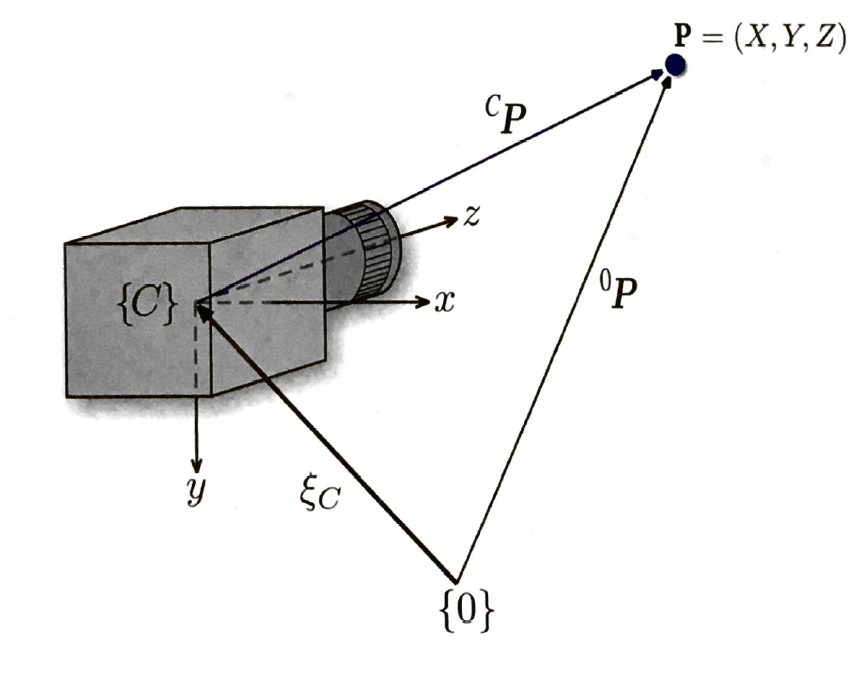
\includegraphics[scale=0.5]{./pics/cameraCoordinateFrame.png}
\caption{camera coordinate frame\cite{Corke}.}
\label{fig:cameraFrame}
\end{center}
\end{figure}

Or by using the homogenous coordinates 
\begin{equation}
{}^{c}\textbf{P}=\textbf{T}_c^{-1}\, {}^{0}\textbf{P}
\end{equation}

\subsubsection{Discrete image plane}
As shown on fig \ref{fig:projectionModel} the image plane in a digital camera constructed by $ W\times H $ photosites, which is light-sensitive elements, that correspond to pixels of the image.  The positive pixel coordinate system is a 2-vector $(u,v)$ and the origin is at the top-left hand corner of the image plane.
The pixel coordinate is related to the image-plane coordinate by
$$\frac{x}{\rho_w} + u_0, v = \frac{y}{\rho_h}+v_0$$
$\rho_w : $ width of each pixel
\\
$\rho_h : $ height of each pixel
\\
$(u_0,v_0) : $ principal point
\\

We can rewrite the linear perspective projection matrix in terms of pixel coordinates acknowledging the camera parameter matrix  $K$
\begin{equation}
\tilde{\textbf{P}}= \begin{pmatrix}
\frac{1}{\rho_w}&0&u_0\\
0&\frac{1}{\rho_h}&v_0\\
0&0&1\\
\end{pmatrix}\begin{pmatrix}
f&0&0&0\\
0&1&0&0\\
0&0&1&0\\
\end{pmatrix}{}^{c}\tilde{\textbf{P}}
\end{equation}

$\tilde{\textbf{P}}=(\tilde{u},\tilde{v},\tilde{w})$ : is the homogenous coordinate of the world p in the pixel coordinates
\begin{equation}
u= \frac{\tilde{u}}{\tilde{w}}, v= \frac{\tilde{v}}{\tilde{w}}
\end{equation}

$(u,v)$ : nonhomogenous image-plan pixel coordinates

\subsubsection{Camera matrix}
From the previous equation the camera projection equation can be formulated in the general form as
\begin{subequations}\begin{align}
\tilde{\textbf{P}}&= \begin{pmatrix}
\frac{f}{\rho_w}&0&u_0\\
0&\frac{f}{\rho_h}&v_0\\
0&0&1\\
\end{pmatrix}\begin{pmatrix}
1&0&0&0\\
0&1&0&0\\
0&0&1&0\\
\end{pmatrix}{}^{0}\textbf{T}_c^{-1}\tilde{\textbf{P}}\\
\tilde{\textbf{P}}&= \textbf{K}\textbf{P}_0 \,{}^{0}\textbf{T}^{-1}_c\,\tilde{\textbf{P}}\\
\tilde{\textbf{P}}&= \textbf{C}\tilde{\textbf{P}}
\end{align}
\end{subequations}
Where the first two matrices are the intrinsic matrix and last two matrices are the extrinsic matrices.
The projection function can be written as\cite{Corke}
\begin{equation}
\textbf{P}=p(\textbf{P},\textbf{K},\varepsilon_c)
\end{equation}
$\textbf{K}$ : camera parameter matrix
\\
$\varepsilon_c$ : camera pose\\
The camera Parameter matrix K includes the characteristics the camera and the sensors like $f,\rho,\rho_h,u_0  and v_0$. Furthermore, the pose of the camera holds the six extrinsic parameters that describe camera orientation and translation.
\\
We have a total of 11 independent parameters to describe a camera, 5 intrinsic and 6 extrinsic parameters. In practical life, the camera parameters are not known and must be calculated by using a camera calibration process, which will be explained in the calibration section.
\\
The camera field of view is a function of its focal length f  and dimensions of the camera chip $W\rho_w  \times  H\rho_h$. The field of can be determined from the geometry of fig \ref{fig:projectionModel}.
In the horizontal direction the angle of view is calculated as following.
\begin{equation}
\theta_h = 2\arctan{\frac{{W_\rho}_w}{2f}}, \theta_v = 2\arctan{\frac{{H_\rho}_h}{2f}}
\end{equation}
$W: number of pixels in the horizontal direction$


\subsubsection{Lens Distortion}
As mentioned in the introduction, that no lens is perfect due to many factors. Lens imperfection leads to a geometric distortion, where points on the plane are not displaced where they should be.
\\
The geometric distortion is one of the most famous distortion effects that is comprises two components, the radial and tangential distortion. The Radial distortion is the displacement of the image points along radial lines from the principal point. The radial error can be approximated through the polynomial as following 
\begin{equation}
\delta_r=k_1r^3+k_2r^5+k_3r^7+...
\end{equation}
$r:is the distance of the image point from the principal point$
The decentering distortion or the tangential distortion, occurs at the right angle to the radii but it's not stronger than radial distortion.
The can describe the coordinate of the distorted matrix as following 
\begin{equation}
u^d = u+\delta_u,v^d=v+\delta_v
\end{equation}
The displacement matrix is like the following, where the first matrix is describing the radial distortion and the second matrix describes the tangential distortion\cite{Corke}.
\begin{equation}
\begin{pmatrix}
\delta_u\\
\delta_v\\
\end{pmatrix}=\begin{pmatrix}
u(k_1r^2+k_2r^4+k_3r^6)\\
v(k_1r^2+k_2r^4+k_3r^6)\\
\end{pmatrix}+\\
\begin{pmatrix}
2p_1uv+P_2(r^2+2u^2)\\
p_1(r^2+2v^3)+2P_2uv
\end{pmatrix}
\end{equation}
In practical life to describe the radial distortion only three coefficients are sufficient and the distortion model is parameterized by $(k_1,k_2,k_3,p_1,p_2)$. Which are considered as additional intrinsic parameters.

\subsubsection{Calibration with checkerboard}
Based on a popular Toolbox for calibrating cameras, which is presented from Caltech university.By using a chessboard, where several images of calibration patterns, always between 10 to 20 images. The images have been taken at different distances and orientations as shown in the following figure.
%Chessboard pic
\\
To pass the images to the toolbox, so they had to use an uncompressed images or loss less compression formats such as PNG. Since the default format of a USB Webcam is JPG, so we hat to convert the images to PNG format. Moreover, we hat to measure the exact length of one side of a square from the checkerboard pattern to improve the process accuracy. After passing the patter images to the Toolbox, an image analyzing process starts to analyze each image, so it detects if the image is duplicated or if the entire chessboard could not be detected because of blurry images or an extreme angle of the pattern.

\subsubsection{Canny and Sobel edge detection}
To perform camera calibration and to calculate the distortion for each pixel, so the camera will be stimulated with vertical and horizontal line at each position. In deed to detect line from a displayed image and to cancel all environment noises we must perform image processing and extract image primitives of interest. 
To extract lines, we should look for regions where strong change of intensity or color in the processed Image. In that section, we will compare many different predefined line detection algorithms and choose the best algorithm that suits our requirements.

\subsubsection{Sobel operator}
The main idea of the Sobel operator or Sobel filter is that it affects the vertical or horizontal image frequencies based on which kernel is used, therefore Sobel operator is considered as directional filter. On the other side Sobel operator is a gray scale operator so we've to convert the image to gray scale before applying the algorithm\cite{Langaniere}.
\\
The Sobel operator uses two Kernels that operates on each pixel that have the following form to calculate the derivatives of Intensity function\cite{Langaniere}.
\begin{equation}
Kernel_{vertical}=\begin{pmatrix}
-1&0&1\\
-2&0&2\\
-1&0&1\\
\end{pmatrix}
\end{equation}
\begin{equation}
Kernel_{horizontal}=\begin{pmatrix}
-1&-2&-1\\
0&0&0\\
1&2&1\\
\end{pmatrix}
\end{equation}
\begin{equation}
grad(I)=\begin{bmatrix}
\frac{\partial I}{\partial x},\frac{\partial I}{\partial y}
\end{bmatrix}^T
\end{equation}

%Sobel Figure

Since the calculated gradient lines at each pixel has a x and y direction, so it's interesting to calculate the norm and direction to get the amplitude of the variation and the orientation.
\begin{equation}
|grad(I)|=\sqrt[2]{\left(\frac{\partial I}{\partial x}\right)^2+\left(\frac{\partial I}{\partial y}\right)^2}
\end{equation}
\begin{equation}
\theta_{orientation}=\arctan{\frac{\partial I}{\partial y},\frac{\partial I}{\partial x}}
\end{equation}
%Soble figutre Orientation 
After applying Sobel operator, we can conclude that this algorithm detects a lot of edges, which is not the actual edge because of the small kernel. Therefore, the algorithm is noisy. 
\subsubsection{Canny operator}
The Canny operator is based on Sobel operator and it is very useful to remove the edges that we are not interested in.  Simply Canny operator takes the output of Sobel operator. 
\\
The Canny operator start working on images after many stages. Firstly, the Image should be converted to grayscale Image. After that the gaussian blur filter is applied.   Hereafter the Soble operator is applied on vertical and horizontal directions. At the end, the calculation of the orientation is to be done to get ready to apply Canny operator.
\\
The most powerful part of that method is the hysteresis thresholding: The hysteresis thresholding is defined as two thresholds, min thresholds and max thresholds. The thresholds classify the strong edges,which is a main edges of an object. form weak edges.  So, any edge above the top threshold will be taken and anything under the lower threshold will be ignored. The region in between will be inspected, that any strong edge is connected to edge at that region by pixel traversal will be included.
















\section{Mapping of correspondencing pixels}
\label{sec:mapping}
Our aim was to create a map of corresponding pixels of the screen to the camera image. For that we followed different approaches which we evaluate by accuracy in Chapter \ref{sec:results} and by runtime in Chapter \ref{sec:runtime}. \\
Before we begin with the mapping of the correspondencies we will discuss the setup of the device. The camera should be in a distance to the screen that it only detects the screen and nothing else like the borders or so. We should be able to manipulate the entire visible flat surface to excite every pixel on the camera image. The background color of the monitor should be black so that drawn white pixels can be better recognized. The camera and the display should be in a locked dark area where no light is coming so the monitor is the only light source. This leads to no unwanted reflections that sophisticate our result. If the camera is adjusted perpendicular to the display the program could run.
\begin{figure}[h]
\begin{center}
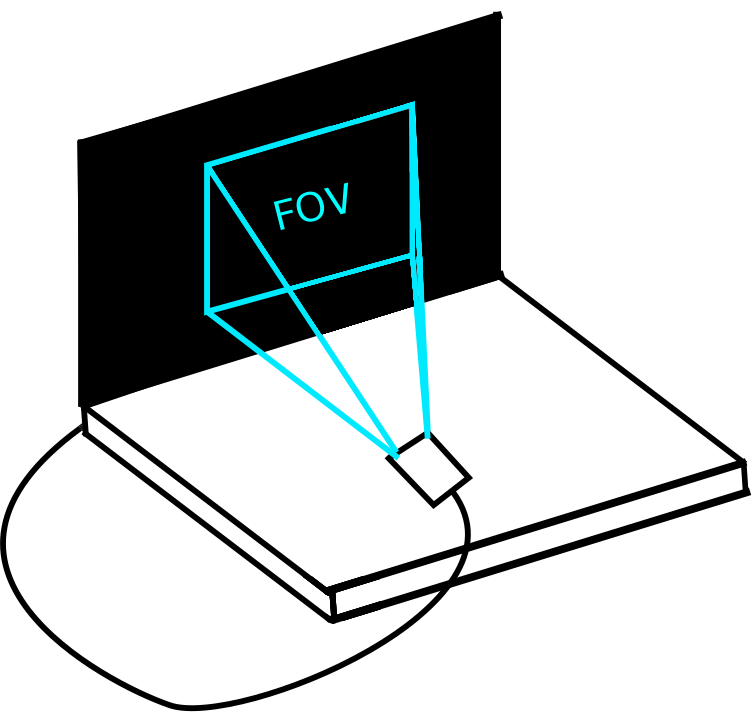
\includegraphics[scale=0.25]{./pics/setup.png}
\caption{Setup of Camera and Monitor}
\label{fig:setup}
\end{center}
\end{figure}\\
 First we have to make sure, that the captured image contains at least one position at which the screen is going to display a rectangle. To do this we draw a set amount of rectangles evenly spaced on the screen. Initially these rectangles have a \emph{width} and \emph{height} of $1$. While the camera doesn't detects a pixel we increase \emph{width} and \emph{height} of the drawn rectangle by $1$ until it does recognise a drawn pixel. This is shown in algorithm~\ref{algo:pixelsize}. In order to ensure, that the detection was not a accidental chance of luck, the same size has to be confirmed by further detections. 
\begin{algorithm}[h]
 \KwData{cameraImage}
 \KwResult{returns pixelSize}
 initialization: int pixelSize = 1\;
 \While{(notDetected)}{
  \eIf{(maxBrightnestPixel != 0)}{
   notDetected = false\;
   return pixelSize\;
   }{
   notDetected=true\;
   pixelSize++\;
  }
 }
 \caption{pixel size detection}
 \label{algo:pixelsize}
\end{algorithm} 
 
 After the pixel size that is seen by the camera is detected we draw a pixel with that size on the screen that is moving with a spacing. That means that the pixel always gets a new coordinate that with a calculated distance in vertical and/or horizontal  direction. Therefore we're able to calculate an optimal spacing for a specific method of us which is described at the end of Chapter \ref{sec:linebased}. While the pixel is moving on the screen we accumulatively add the $x_s$ and $y_s$ positions of the seen rectangles on the screen. Simultanously we enumerate the number of seen rectangles. The algorithm is shown in \ref{algo:centerPoint}.
 
\begin{algorithm}[h]
 \KwData{pixelPosition}
 \KwResult{returns centerPoint}
 initialization: int counter = 0\;
 \While{(pixelPosition < display)}{
  \eIf{(pixelSeen)}{
   centerPoint += pixelPosition\;
   counter++\;
   }{
   centerPoint /= counter\;
   }
 }
 \caption{calculation of center point of FOV}
 \label{algo:centerPoint}
\end{algorithm} 

As you will see in the following chapters, these two methods are fundamental to most of our approaches. Where the pixelSize is not necessary for the algorithm itself, we still use it to generate a test image. To this test image the found distortion maps are applied. Therefore they are necessary in any case. In the next three Subchapter we'll present two principle different possibilities we obtained while this work how it could be possible to get a distortion calibration with a higher accuracy than the state of the art. 

\subsection{Pixelwise approaches}
Our first idea was a matching from every screen pixel to his corresponding pixel in the image. We developed three different methods. These were faster in their implementation in this order, with the same accuracy. The duration of the individual methods is given in Chapter \ref{sec:runtime} with an exact minimum value for our example.
\subsubsection{every Pixel}
The first and easiest idea was to light a rectangle with minimum pixel size after another and row for row. If we see a drawn rectangle save the correspondencies of the image and the screen coordinate. Later we could have checked if an imaginary straight line of rectangles on the screen will be to a straight line of pixels on the image. If not we knew we have to move the image pixels so that the line that is seen on the image is also straight.
\subsubsection{For the sake of the \textbf{SPIRAL}}
However it's not very efficient if we light every pixel of the screen with the seen pixel size. As the seen area on the screen the field of view (FOV) could be significant smaller than the screen we developed another method to ensure a faster result. For this purpose we produce generate the idea to let the rectangle move on a spirallike path on the screen. The algorithm \ref{algo:centerPoint} was designed to find a optimal starting position to that spiral. After finding the center point of the FOV the rectangle moved slowly to the outside of the FOV. While the pixel wasn't seen for a hole circulation we know we should still be in vision of the camera. So everytime a rectangle is seen it's position on the screen and the camera image is saved for later for the distortion calibration. Exposing the view area in spiral-shape, as described in Chapter \ref{sec:runtime}, is not exactly fast. In addition, the method is very inefficient for fisheye cameras or any kind of wide angle cameras. 

%% mathematics and basics -> some pictures with different distortion shapes
\subsubsection{by lines}
The pixelwise distortion calibration was our last concept in which we tried to detect a solution by lighting several rectangles with the minimum pixel size. However this method is already a hybrid since we introduced real line detection methods here to solve the problem of distortion calibration. In the further discussed methods we used the pixel correspondencies and calculated the lines in both images, the drawn and the detected one. In this method we drew lines in the seen area and detect their position in the camera image and wanted to correct them then. However we need to detect the borders of the seen area first. For that we are forced to find at least one border of the seen area. Therfore we developed a binary search algorithm that finds a border. The initial point to that algorithm is the center point we already detected with algorithm~\ref{algo:centerPoint}. From there we assumed that a point at any border of the screen is not seen by the camera. Then we check if a point between this two points is seen or not. If not we check between this and center point and else we check between that and the point of the border. This is described in algorithm~\ref{algo:binary}. 


\begin{algorithm}[h]
 \KwData{pixelPosition}
 \KwResult{returns borderPoint}
 initialization: \;
 point lastSeen = centerPoint\;
 point lastNotseen = screenBorder\;
 point nextPos\;
 \While{(abs(lastSeen - lastNotSeen)>1)}{
 nextPos = (lastSeen+lastNotSeen)/2\;
  \eIf{(pixelSeen)}{
   lastSeen = pixelPosition\;
   }{
   lastNotSeen = pixelPosition\;
   }
 }
 pixelPosition = nextPos\;
 return borderPoint = (lastSeen+lastNotSeen)/2\;
 \caption{binary search algorithm for border detection}
 \label{algo:binary}
\end{algorithm} 
In the process of this work the binary search showed that absolute darkness around the setup is necessary because otherwise we're losing vision on pixels in the outer area of the camera image. \\After a border is found our purpose was to find all corresponding screen pixels that belongs to the frame of the camera image. If these are found our idea was to draw lines with \emph{width} for vertical lines and the \emph{height} for horizontal lines of the minimum pixel size on the screen that are straight. Then we should have been able to calibrate the distortion with the next two shown images. However it would have needed still a long time to detect the borders. Since around a pixel 8 possible positions to detect the next one that belongs to the frame exist. Even if you can exclude some of these possible positions if you know at which border you are and in which directions you want to move around the frame, at least 4 possible positions remain. %% Picture Positions? 
In Chapter \ref{sec:runtime} we calculated the minimum time required for an exemplary FOV. However we dismissed this method too because we found a way faster solution with a line detection by a \emph{openCV}--function called \emph{Canny}. 

\subsection{simple linedetection for x and y matching}

\begin{figure}[h]
\begin{center}
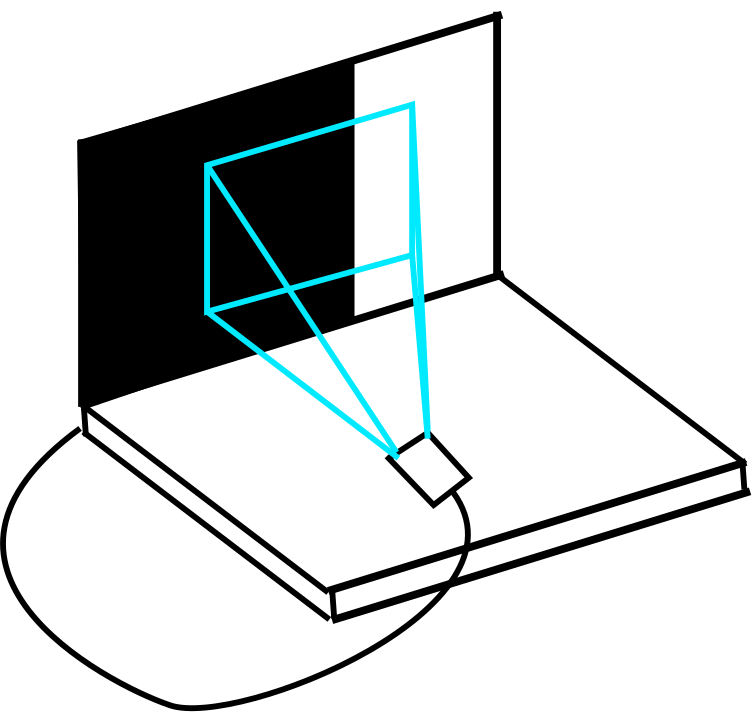
\includegraphics[scale=0.25]{./pics/rect.png}
\caption{rectangle over the screen}
\label{fig:setup}
\end{center}
\end{figure}

We set the backround of the screen to black. Then we draw a white rectangle with height of the screen height and an increasing width. In figure \ref{fig:blockOverTime} we show how the rectangle is getting wide. At the border of the white rectangle to the black backround the \emph{Canny}-operator detects the points of the border as a line. The return of that operation is a point cloud of image coordinates that belong to that line. To every image pixel that in that point cloud we match the $x$--coordinate to which it should belong. We enlarge the width of the rectangle until it disappears from the FOV. After that we do the same with another rectangle that is as width as the screen width and height of one minimum pixel size \emph{height}. We'll get again every pixel that belongs to that line in a point cloud by the \emph{Canny}--operator. Now we can match the $y$--coordinates to the points which are obtained, since they always belong to the actual drawn line. At the end of Chapter \ref{sec:runtime} we calculated the runtime of this method. It is significantly faster than any of the other methods we have presented so far. However, it can be accelerated even more, if not always a pixel size is increased, but several. Therefore we wrote a interpolation function that interpolates linearily between matched pixels. In future it could be tested if another interpolation method besides linear interpolation give better results. In case of radial distortion a radius to the center point dependent interpolation could return better results.
\\

\begin{figure}[h]
\begin{center}
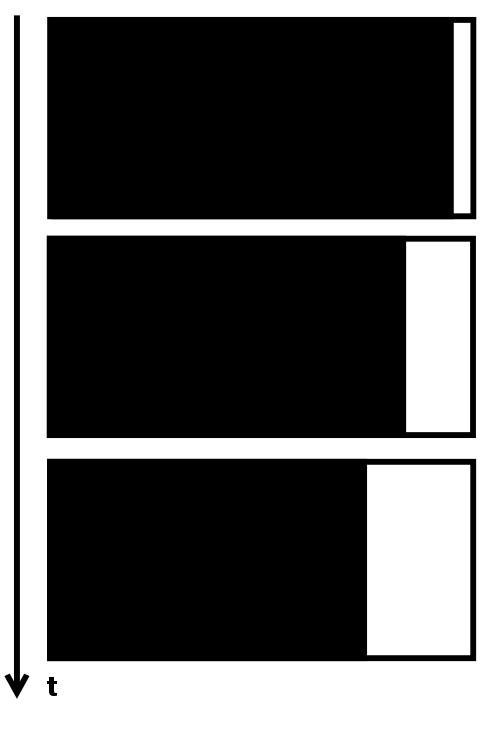
\includegraphics[scale=0.3]{./pics/pattern.png}
\caption{Rectangle over time}
\label{fig:blockOverTime}
\end{center}
\end{figure}

\subsection{runtimes and seen area}
\label{sec:runtime}
\subsubsection{Field of View}
\label{sec:FOV}
Each frame makes one call to the draw function. Given that we need 7 calls of the draw function to fully draw, capture, and process one image, we can, with a frame rate of $21$ frames per second, achieve turnover rate of $3$ images per second. This allows us to make an estimation of the runtime of each approach we tested out or considered for the lens calibration based on the amount of necessary images. The runtime $rt$ of the program could be calculated as shown in the following Chapter. 
\begin{align}
rt(noImages) = \frac{1}{3} \cdot noImages 
\end{align}
To determine the amount of images for some methods, we need an estimate of the field of view. In order to estimate the FOV we used a simple method with a measuring tape. The only further information necessary, is the amount of pixels per inch ($ppi$) of the used screen. By placing the measurement tape flat on the screen, we can measure the width and height visible in the captured image. The measurement has then to be converted to inches in order to calculate the amount of pixels. The conversion constant from centimeters to inches is roughly $0.3937$. Multiplying this with the ppi yields the pixels seen. Let $l$ be the length of the visible measurement tape in centimeters, then the amount of pixels in the FOV can be calculated as:
\begin{align}
FOV(l) = ppi \cdot 0.3937 \frac{inch}{cm} \cdot l .
\end{align}
From this we can also calculate the diagonal aperture angle of the camera. By comparing the calculated angle with the angle from the specifications of the camera, we have an estimation about the accuracy of the calculated FOV. If the diagonal aperture angles are differ largely, our estimation is inaccurate. If they are similar, it is acceptable.\\
To calculate the aperture angle $\alpha$ for the width or height $\left( \alpha_{width||height}\right)$, we also need the distance $d$ of the camera to the screen. The distance and FOV dimensions need to be used with the same unit. From there the aperture angle is simple trigonometry, see image ... .
\begin{align}\begin{split}
&\frac{1}{2}\cdot\alpha_{width||height}  =  \arctan \left(\frac{FOV_{width||height }}{2\cdot d} \right),
\end{split}
\end{align}
\begin{align}\begin{split}
\Rightarrow &\alpha_{width||height} = 2 \cdot \arctan \left(\frac{FOV_{width||height }}{2\cdot d} \right),
\end{split}
\end{align}
\begin{align}\begin{split}
&\alpha_{diag} = \sqrt{\alpha_{width}^2 + \alpha_{height}^2)}.
\end{split}
\end{align}
In our setup we used an \emph{ASUS--VX239} screen of dimensions $1290$x$1080$ pixels and $95.78~ppi$ and a \emph{Microsoft~LifeCam~HD--3000}. We weren't able to place the camera exactly perpendicular to the screen. This warps the FOV somewhat. Therefore we used an average of the largest and smallest measurement of the FOV width and height. On average we measured a width of $17.75~cm$, and a height of $10.45~cm$. This yields us FOV dimensions of
\begin{align*}
FOV_{width}(17.75~cm) \approx 669.327~pixels
\end{align*}
\begin{align*}
FOV_{height}(10.45~cm) \approx 394.050~pixels
\end{align*}
Since we would rather overstate the runtime than understate it, we used $670$ pixels for the width and $395$ for the height. The distance between camera and screen was roughly $16.0~cm$. This yields aperture angles of:
\begin{align}\begin{split}
\alpha_{width}(17.75~cm)&= 2 \cdot \arctan\left(\frac{17.78~cm}{2 \cdot 16~cm}\right) \\&= 58.12^{\circ}\end{split},
\end{align}
\begin{align}\begin{split}
\alpha_{height}(10.45~cm) &= 2 \cdot\arctan\left(\frac{10.45~cm}{2 \cdot 16~cm}\right) \\&= 36.17^{\circ}\end{split},
\end{align}
\begin{align}\begin{split}
\alpha_{diag} &= \sqrt{58.12^2 + 36.17^2} \\& \approx 68.46^{\circ}.\end{split}
\end{align}
The specifications for the camera state a diagonal aperture angle of $68.50^{\circ}$. Judging from the difference of roughly $0.04^{\circ}$, this should be close enough to the true FOV dimensions to use it for runtime estimations.Furthermore the assumption is made that each pixel can be detected on its own, instead of needing larger patches to be detectable by the camera.\\
The following variables will be use: $h_{FOV}$ as the height of the FOV, $w_{FOV}$ as the width of the FOV, $w_s$ as the width of the screen, and $h_s$ as the height of the screen.\\
\subsubsection{Singular pixel detection}
\label{singlePixel}
With a naive approach each patch of minimal detectable size on the screen has to be turned on separately.
\begin{align}
rt(w_s, h_s) = \frac{1}{3} \cdot w_s \cdot h_s
\end{align}
This means screen width times screen height necessary images. In our set up $921,600$ images would be needed, yielding a runtime of $307,200$ seconds, or $3$ days $13$ hours $20$ minutes.\\
It can be sped up however. . By lighting up single pixels in a spiral pattern around an estimation of the middle point, the amount of images can be reduced to the amount of pixels within the camera’s FOV plus one pixel in each dimension. The additional pixel is necessary, because it allows us to know, when the spiral does not need to actually be done, but can jump to a next position. This is due to the pixel outside no longer being detected. \begin{align}
rt(w_{FOV}, h_{FOV}) = \frac{1}{3} (w_{FOV} + 1) \cdot (h_{FOV} + 1)
\end{align}
In our setup, we need 265,716 images, leading to a runtime of 88,572 seconds, or 1 day 36 hours 12  seconds. The center point estimation has been left out, as it is comparably negligible.\\
	
\subsubsection{Line-based detection} 
\label{sec:linebased}
The first idea for a line-based detection was to first detect the borders and store how the border pixels of the image map to the screen. The idea was to first detect a pixel on the border via binary search and then move this pixel to new positions to check whether these are seen. We need to check at least four surrounding pixels for visibility.  For the runtime of only the border detection, once the binary search is done, this means 
\begin{align}
rt(w_{FOV}, h_{VOF}) = \frac{4}{3} (2 \cdot h_{FOV} + 2 \cdot w_{FOV})
\end{align}
In our setup, we need $8,520$ images, leading to a runtime of $2,840$ seconds, or $47$ minutes $20$ seconds.  After discovering the border only two images need to be created and processed. However, since the discovery of the border would take still too long, we rejected this method as well.\\
The next method is a segmentation of the screen. By segmenting the screen sequentially in a black and a white part, we can detect a single edge in the image. The white part starts out as the entire screen and gradually decreases in width, pixel by pixel. After that is done, the white part is again stretched out over the entire screen and then decreases in height. At each image we know exactly at which position the screen shows the edge. From this we can calculate where the edge pixels from the image should have appeared.\\
A naïve and simple approach is to go over the entire screen width and height. Each row and each column is once the edge row or column. This leads to a runtime of
\begin{align}
rt(w_s, h_s) = \frac{1}{3} (w_s + h_s)
\end{align}
In our setup, we need $2,370$ images, leading to a runtime of $790$ seconds, or $13$ minutes $10$ seconds.  This is already immensely faster. It can still be sped up, however.\\
Instead of going over the entire screen, we first estimate the center point again. This time we additionally store which was the outermost pixel, which was visible during the estimation, for each border. From there we add the spacing, that was used, plus a small margin to be safe. The margin was chosen to be $5$ pixels wide. In this method the runtime for the center point estimation is relevant. While the runtime for the center point estimation increases with smaller spacing, the runtime for the line-based detection decreases. This means a runtime-optimal spacing can be calculated.\\
Let s be the spacing between the positions of the pixels to be lit, and m the margin. Then the runtime of the center estimation, as a function of spacing s, is:
\begin{align}
rt_c (s) =\frac{1}{3} \frac{w_s\cdot h_s}{ s^2} =\frac{1393200}{3s^2} .
\end{align}
For the runtime of the line-based detection after that, follows:
\begin{align}\begin{split}
rt_d (s) &=\frac{1}{3}\left( 4s + 4\cdot m + w_{FOV} + h_{FOV}\right)\\& = 4s + 1085\end{split}
\end{align}
From there the overall runtime can be calculated as:
\begin{align}\begin{split}
rt(s) &=\frac{1}{3}\left(\frac{w_s*h_s}{s^2} + 4s + 4m + w_{FOV} + h_{FOV}\right)\\& = \frac{\frac{1,393,200}{s^2} + 4s +1085}{3}.\end{split}
\end{align}
For calculating the minimum of this function we take the first derivative w.r.t. spacing s and set it to zero:
\begin{align}\begin{split}
&rt’(s) = \frac{1}{3} \cdot \left( \frac{-w_s \cdot h_s}{s^3 }  + 4\right) = \frac{ \frac{-1,393,200}{s^3}+ 4}{3},\\
\Rightarrow &s = \sqrt[3]{\frac{w_s * h_s}{4}} = \sqrt[3]{\frac{1393200}{4}}. \end{split}
\end{align}

The functions minimum is at roughly $s = 70$. For this spacing we need then $1,650$ images, leading to a runtime of $550$ seconds, or $9$ minutes $10$ seconds. Of these roughly $1$ minute $35$ seconds are taken by center point estimation.\\
If this is deemed too slow, but the restriction of true pixelwise mapping is lifted, it can be sped up. We skip a set amount of pixels, when moving the white rectangle over the screen. We can introduce the jump width as variable $j$, i.e. every $j$--th pixel will be part of an edge. This changes our runtime formula for the detection part to, when assuming the same margin $m$:
\begin{align}\begin{split}
rt_d (s; j) &=\frac{1}{3} \cdot \frac{4*s + 4 * m + w_{FOV} + h_{FOV}}{j}\\
 &= \frac{4s + 1085}{3j},\end{split}
\end{align}
and thus the overall formula and its derivative to:
\begin{align}\begin{split}
rt(s; j) &= \frac{1}{3} \left(\frac{w_s\cdot h_s}{3} + \left( 4s + 4m + w_{FOV} + h_{FOV}\right)\frac{1}{j}\right)\\ &=\frac{1}{3}\left( \frac{1,393,200}{s^2} + \frac{4s +1085}{j}\right),\end{split}
\end{align}
\begin{align}\begin{split}
rt’(s; j) &= \frac{1}{3} \left(\frac{-w_s * h_s}{s^3} + \frac{4}{j}\right)\\& =\frac{-1,393,200 }{3s^3} + \frac{4}{3j} \end{split}
\end{align}
The new optimal spacing is now calculated as:
\begin{align}\begin{split}
s &= \sqrt[3]{\frac{w_s \cdot h_s \cdot j }{ 4}} \\&= \sqrt[3]{\frac{1,393,200 * j} { 4}}.\end{split}
\end{align}
For a skip of $j = 3$ we get in our setup an optimal spacing of roughly $s = 101$. This spacing and skipping, we need $633$ images, leading to a runtime of $211$ seconds, or $3$ minutes $31$ seconds. Of these roughly $46$ seconds are taken by center point estimation.




\section{results}
\label{sec:results}
\subsection{accuracy}
\subsection{comparation and valuation}

\section{Problems}
\label{sec:probs}
Several problems appear during the process of this project.
The first is the use of new programming tools. Openframeworks is a toolkit with powerful embedded functions (setup(), update() and draw()) which has an advantage that draws parallel to processing, however, it brings timing issues in our project, since the update function only runs once before drawing. Getting rid of it costs the first several weeks and slowed the process down. Ultimately we divided each app into several states in draw(), and use a state machine to control the process, which turns out to be a good solution.  \\
The next problem is, several classes with their own functions has been written to achieve a modularly structured program. A  master--class was created to bring these module--classes and their functionality together. So each module--class brings a functionality and together they solve th our problem to undistort a image. This splitting of the code made it necessary to retain information gained in each part. This, however, was a problem. Any class that is supposed to draw on the screen, needs to inherit from openframeworks class ofApp. Any class that inherits from class ofApp, has to be started with the openframeworks function ofRunApp.\\
While the runtime of each App, the only way to access data is to work with multi-threading and trying to access variables from another thread. Since it have to be ensured, that there are no read/write access violations and that the threads are properly synchronized, this method is problematic. \\
There is also a problem to access information after the runtime of the apps, since after the runtime of the app all variables used within are deleted. To overcome this disadvantage, a pointer of the app is introduced to a variable outside of it. This ensured that the app wrote into that variable. Since the variable wasn't within the scope of the app, the information in it was retained even after the app was closed and deleted.\\
The modular program structure was important for us, as we wanted to keep an overview of the code itself. It also allows functionalities easily replaceable as long as the defined interfaces are kept the same.
\\
We also set ofSetBackgroundAuto(false) to avoid flickering of the screen, which brings has problematics since for Windows 10 systems because of incompatibility. 




%\bibliography{literatur}

\begin{thebibliography}{1}
\bibitem{Zhang}
Zhang and Zhengyou. \emph{A flexible new technique for camera calibration}, p.965--980, vol.14 num.10, IEEE Transactions on Pattern Analysis and Machine Intelligence, 2010

\bibitem{Sturm}
P.F.~Sturm and S.J.~Maybank. \emph{On plane-based camera calibration: A general algorithm, singularities, applications}, Computer Vision and Pattern Recognition, IEEE Computer Society Conference on. IEEE, p.432--437, 1999

\bibitem{Faugeras}
O.~Faugeras, Q.T.~Luong and S.~Maybank. \emph{Camera self-calibration: Theory and experiments},p. 321--334Computer Vision--ECCV'92, 1992

\bibitem{Ma:2010}
Y.~Ma. \emph{{An invitation to 3-D vision: From images to geometric models}, {Springer} , {978-1-4419-1846-8}}

\bibitem{Sagawa}
R.~Sagawa and M.~Takatsuji and T.~Echigo and Y.~Yagi . \emph{Calibration of lens distortion by structured-light scanning} IEEE/RSJ International Conference on Intelligent Robots and Systems, p.832--837 , 2005

\bibitem{Salvi}
J.~Salvi and J.~Pag{\`e}s and J.~Batlle. \emph{Pattern codification strategies in structured light systems}, vol.37 num.4, Pattern Recognition, p. 827--849, 2004

\bibitem{Swaminathan}
R.~Swaminathan and S.K.~Nayar. \emph{Nonmetric calibration of wide-angle lenses and polycameras}, p.1172--1178, vol.22 num.10, IEEE Transactions on Pattern Analysis and Machine Intelligence

\bibitem{Weng}
J.~Weng and P.~Cohen and M.~Herniou. \emph{Camera calibration with distortion models and accuracy evaluation}, p.965--980, vol.14 num.10, IEEE Transactions on Pattern Analysis and Machine Intelligence, 1992

\bibitem{Duane}
C.B.~Duane  \emph{Close-range camera calibration}. Photogramm. Eng, vol.37 num.8, p.855-866. 1971


\end{thebibliography}

\begin{biography}[{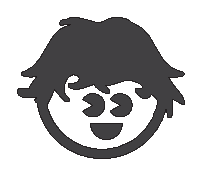
\includegraphics[width=1in,height=1.25in,clip,keepaspectratio]{./pics/ComicKopf.eps}}]
{Ahmed Ashraf} is from egypt. He likes sport and Matlab.
$\cdots$
\end{biography}
\begin{biography}
[{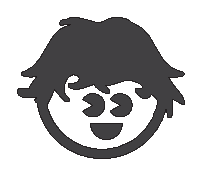
\includegraphics[width=1in,height=1.25in,clip,keepaspectratio]{./pics/ComicKopf.eps}}] % hier ein Foto einbinden
{Nils Hamacher}
Biographie Autor B.
\end{biography}
\begin{biography}
[{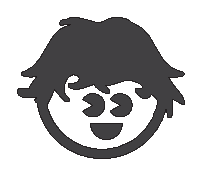
\includegraphics[width=1in,height=1.25in,clip,keepaspectratio]{./pics/ComicKopf.eps}}] % hier ein Foto einbinden
{Linhan Quan}
Biographie Autor C.

\end{biography}

\begin{biographynophoto}
%[{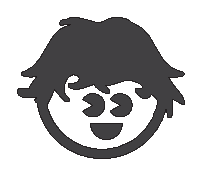
\includegraphics[width=1in,height=1.25in,clip,keepaspectratio]{./pics/ComicKopf.eps}}] % hier ein Foto einbinden
{Vivica Wirth}
Biographie Autor D.

\end{biographynophoto}

\end{document}
